%%%%%%%%%%%%%%%%%%%%%%%%%%%%%%%%%%%%%%%%%%%%%%%%%%%%%%%%%%%%%%%%%%%%%%%
% Universidade Federal de Santa Catarina
% Biblioteca Universitária
%
% (c)2010 Roberto Simoni (roberto.emc@gmail.com)
%         Carlos R Rocha (cticarlo@gmail.com)
% ---------------------------------------------------------------------
% Alterações:
% 2018 Rafael Crispim Ignácio (rafael.nacio@gmail.com)
%%%%%%%%%%%%%%%%%%%%%%%%%%%%%%%%%%%%%%%%%%%%%%%%%%%%%%%%%%%%%%%%%%%%%%%

%\PassOptionsToPackage{abnt-etal-cite=1, abnt-etal-list=0}{abntcite}
\documentclass{ufscThesis}

%%%%%%%%%%%%%%%%%%%%%%%%%%%%%%%%%%%%%%%%%%%%%%%%%%%%%%%%%%%%%%%%%%%%%%%
% Pacotes usados especificamente para este documento
% Definidos pelo criador do documento
%%%%%%%%%%%%%%%%%%%%%%%%%%%%%%%%%%%%%%%%%%%%%%%%%%%%%%%%%%%%%%%%%%%%%%%
\usepackage{graphicx, tikz, mathtools, multirow, fancyref, float, lscape, longtable}
\usepackage{verbatim}
\usepackage{pdfpages}
\usepackage[portuguese, boxruled, linesnumbered]{algorithm2e}
\usepackage[labelsep=endash]{caption} % O separador de legenda é um -
\usepackage[utf8]{inputenc}
\setlength{\tabcolsep}{18pt}
\renewcommand{\arraystretch}{1.5}

%%%%%%%%%%%%%%%%%%%%%%%%%%%%%%%%%%%%%%%%%%%%%%%%%%%%%%%%%%%%%%%%%%%%%%%
% Identificadores do trabalho

\titulo{Análise de Soluções para Busca por Similaridade ({\itshape Matching}) de Dados Musicais}
\subtitulo{}
\autor{Gisele Bernardes da Silva}
\data{30}{Outubro}{2018}

%----------------------------------------------------------------------
% Orientador, Coorientador e Coordenador

%\orientador[Orientadora]{Profa. Dra. Fulana}
\orientador{Prof. Dr. Ronaldo dos Santos Mello}
%\coorientador{Prof. Dr. Beltrano}
%\coordenador[Coordenadora]{Profa. Senhora, Dra. Eng.}
\coordenador{Prof. Cristian Koliver, Dr.}

%----------------------------------------------------------------------
% Departamento, Curso e Grau

%\departamento[a]{Faculdade de Cięncias do Mar}
\departamento{Departamento de Informática e Estatística}
%\curso[a]{Atividade de Extensăo em Corte e Costura}
\curso{Sistemas de Informação}
\grau{Bacharel em Sistemas de Informação}

%%%%%%%%%%%%%%%%%%%%%%%%%%%%%%%%%%%%%%%%%%%%%%%%%%%%%%%%%%%%%%%%%%%%%%%
% Banca Avaliadora

\numerodemembrosnabanca{5}
\orientadornabanca{nao}
%\coorientadornabanca{sim}

\bancaMembroA{Prof. Dr. Renato Fileto}
\bancaMembroB{Prof. Dr. Raul Sidnei Wazlawick}
%\bancaMembroC{Prof. terceiro membro}
%\bancaMembroD{Prof. quarto membro}
%\bancaMembroE{Prof. quinto membro}
%\bancaMembroF{Prof. sexto membro}
%\bancaMembroG{Prof. sétimo membro}
%%%%%%%%%%%%%%%%%%%%%%%%%%%%%%%%%%%%%%%%%%%%%%%%%%%%%%%%%%%%%%%%%%%%%%%
% Configuração dos elementos pré-textuais

%----------------------------------------------------------------------
% Opcionais - Dedicatória, Agradecimento e Epígrafe

\dedicatoria{Ao meu namorado, por toda paciência, compreensão, carinho e amor.}

\agradecimento{Sou grata aos meus pais, pelo carinho, apoio e amor incondicional. À minha mãe, pela rigidez e educação, pois foram seus ensinamentos que me deram a noção do certo e errado. Ao meu pai, pelo exemplo de esforço e dedicação, por me mostrar que eu sou capaz de trilhar o caminho que desejo e conquistar o que almejo.

Sou grata ao meu namorado, por todo o apoio, paciência, compreensão da minha ausência em horas de estudo, carinho e amor. Por ser gentil, amoroso e por me mostrar que a vida é bela quando se ama.

Sou grata aos meus amigos, pelo companherismo, alegrias, tristeza e principalmente pela amizade. Foi a cumplicidade do dia-a-dia de vocês e o nosso esforço como equipe que me ajudaram a chegar aonde cheguei.

Sou grata à universidade pela oferta do curso e à oportunidade de fazer parte da família nesse período de aprendizado.

Sou grata aos professores, pelo tempo e esforço em compartilhar todo o seu conhecimento, em especial ao meu orientador, pelo empenho dedicado à elaboração deste trabalho.

Sou grata a todos que direta ou indiretamente fizeram parte da minha formação.

Por fim, sou grata à Deus, pela oportunidade de estar nesta Terra e de poder conviver com essas pessoas, sempre aprendendo e evoluindo.}

\epigrafe{Happiness can be found, even in the darkest of times, if one only remembers to turn on the light.}{J.K. Rowling, Harry Potter and the Prisoner of Azkaban}


%----------------------------------------------------------------------
% Resumo

\textoResumo {O som não é algo que podemos ver com nossos olhos. Então, o que é som? O som é a variação da pressão do ar. Sendo assim, a forma de produzir um determinado som depende da maneira como a pressão do ar varia. Representar o som numericamente é chamá-lo de dado, e incluir um "significado" implícito nesse dado é gerar informação. Uma informação musical apresenta determinadas especificidades de comportamento na sua produção, objetivação e uso. Assim, a música tem diferentes significações para cada indivíduo. A música era um meio de comunicação exclusivamente presencial e com a evolução dos inventos tecnológicos, a música ultrapassa os limites físicos da mídia, mergulhando no universo digital. Desta forma, o problema de representação e o processo de construção de sistemas de processamento e recuperação musicais agrava-se com a necessidade de desenvolvimento de sistemas com estruturas internas o mais compatível possível com as visões ou desejos dos usuários. Portanto, a relevância deste trabalho contribui, diretamente, para agregar conhecimento com o estudo sobre a recuperação da informação de dados musicais que auxiliarão no desenvolvimento futuro de soluções para busca por similaridade de dados musicais. Especificamente, este trabalho visa apresentar e comparar soluções para recuperação de informação musical. A intenção é analisar soluções que não necessariamente buscam dados musicais apenas através do casamento direto de parâmetros de entrada para a busca, como título da música, palavras-chave ou um áudio com parte da música, mas também através do casamento aproximado (ou similar) destes parâmetros.} 

\palavrasChave {recuperação da informação musical; busca por similaridade; dados musicais.}

%----------------------------------------------------------------------
% Abstract

\textAbstract {Sound is something we can't see. So, what is sound? Sound is the variation of air pressure. The way to produce a certain sound depends the air pressure varies. To represent the sound numerically is to call it data, and to include an implicit "meaning" in this data is to generate information. A musical information presents certain specificities of behavior in its production, objectification and use. Thus, music has different meanings for each individual. Music was a means of exclusively on-site communication and with the evolution of technological inventions, music surpasses the physical limits of the media, plunging into the digital universe. In this way, the problem of representation and the process of construction of musical processing and recovery systems is aggravated by the need to develop systems with internal structures as compatible as possible to the visions or desires of the users. Therefore, the relevance of this work contributes, directly, to aggregate knowledge with the study on the retrieval of musical data information that will aid in the future development of solutions for searching for similarity of musical data. Specifically, this work aims to present and compare solutions for music information retrieval. The intention is to analyze solutions that do not necessarily search for musical data only through direct marriage of input parameters to the search, such as song title, keywords or an audio with part of the song, but also through approximate (or similar) these parameters.}

\keywords {retrieval of musical information; search for similarity; musical data.}


%%%%%%%%%%%%%%%%%%%%%%%%%%%%%%%%%%%%%%%%%%%%%%%%%%%%%%%%%%%%%%%%%%%%%%%
% Início do documento
\begin{document}
%\renewcommand{\listquadroname}{Lista de Quadros}

%----------------------------------------------------------------------
% Elementos pré-textuais
\capa  
\folhaderosto[comficha]
\folhaaprovacao
\paginadedicatoria
\paginaagradecimento
\paginaepigrafe
\paginaresumo
\paginaabstract
\listadefiguras
\listadetabelas

\listadeabreviaturas
%\listadesimbolos
\sumario

%----------------------------------------------------------------------
% Elementos textuais

\chapter{Introdução}
Nós ouvimos uma variedade de sons à todo momento, e vivemos toda a nossa vida rodeados por eles. Sons de portas abrindo e fechando, dos passos, do ruído dos motores dos automóveis, da chuva e da música. O som não é algo que podemos ver com nossos olhos. Então, o que é som?

O som é a variação da pressão do ar. Sendo assim, a forma de produzir um determinado som depende da maneira como a pressão do ar varia. Representar o som numericamente, é chamá-lo de dado, e incluir um "significado" \ implícito nesse dado, é gerar informação.

Uma informação musical apresenta determinadas especificidades de comportamento na sua produção, objetivação e uso, pois a manifestação da música apresenta-se carregada de características próprias. Portanto, a compreensão completa da música está diretamente ligada com o reconhecimento do contexto histórico e social de sua origem, com a interpretação pessoal e individual do ouvinte, e com os aspectos sonoros que a constituem, dessa forma, a música tem diferente significações para cada indivíduo. Assim, a música é uma expressão humana construída socialmente e objetivada através de sua comunicação oral, registro sonoro ou representação gráfica.

Até o surgimento dos inventos tecnológicos, a música era um meio de comunicação exclusivamente presencial. Com o decorrer do tempo as técnicas e invenções aplicadas ao processo de gravação do som foram surgindo e se aperfeiçoando, resultando em aparelhos reprodutores e suportes cada vez mais versáteis e manipuláveis. A música se tornou um objeto de consumo universal e extremamente acessível.

Com a internet, a música ultrapassa os limites físicos da mídia, mergulhando no universo digital, a música passa a circular livremente pela rede mundial de computadores através do \textit{streaming} e a popularização dos aplicativos que oferecem mais de 30 milhões de música a seus usuários.

Desta forma, a organização da informação, que inclui a sua representação, tem a principal finalidade de possibilitar a recuperação dessa informação, além da sua guarda para a posteridade. A busca por similaridade musical está inserida dentro de um tema de estudos denominado \textit{Music Information Retrieval}. Sua produção se intensificou com a explosão do interesse em coleções em rede que contenham obras musicais na forma digital, possibilitadas pelo desenvolvimento da compressão de áudio. Os pesquisadores de MIR observam que a motivação maior para essa área de pesquisa é o grande volume de música digital disponível na Internet que quanto mais cresce menos possibilita sua recuperação eficiente visto que estão apenas disponíveis aos montes, mas sem o tratamento adequado.

A área de MIR conta com profissionais das mais diversas áreas inclusas na questão do tratamento e recuperação da informação musical, mas não apresenta uma ação interdisciplinar, o que prejudica todo o seu processo de comunicação científica, pois não há um periódico ou livro-texto fundador onde pessoas interessadas podem adquirir as bases teóricas e práticas de MIR. 

Com exceção de alguns pequenos encontros interdisciplinares, muitos pesquisadores estão apresentando seus resultados para membros das suas próprias disciplinas. A literatura de MIR é difícil de ser localizada, lida e estudada, o que dificulta construir e sustentar uma área de pesquisa respeitável e próspera.

Diante das dificuldades provenientes da escassa produção científica a respeito do tema, o problema de representação e o processo de construção de sistemas de processamento e recuperação musicais agrava-se com a necessidade de desenvolvimento de sistemas com estruturas internas o mais compatível possível com as visões ou desejos dos usuários.

Neste trabalho, buscou-se reunir dados/informações com o propósito de contribuir com futuros trabalhos que desejam desenvolver soluções para a busca por similaridade de dados musicais.

Portanto, a relevância deste trabalho contribui, diretamente, para agregar conhecimento com o estudo sobre a recuperação da informação de dados musicais que auxiliarão no desenvolvimento futuro de soluções para busca por similaridade de dados musicais. A pesquisa também tem como objetivo mostrar, de forma clara, o estado da arte sobre a recuperação da informação de dados musicais; Identificar formatos de dados musicais e como é feito o armazenamento deles, no banco de dados; Apresentar métodos e algoritmos utilizados para busca por similaridade de dados musicais; e por fim, apresentar e comparar algumas soluções existentes para busca de dados musicais.

\section{Objetivos}
\subsection{Objetivo Geral}
Este trabalho de conclusão de curso tem como objetivo geral estudar e realizar uma análise comparativa de abordagens para busca por similaridade de dados musicais.

\subsection{Objetivos Específicos}
 \begin{itemize}
   \item Estudar a fundamentação teórica sobre a recuperação da informação de dados musicais;
   \item Identificar formatos de dados musicais e como é feito o armazenamento deles, no banco de dados;
   \item Apresentar métodos e algoritmos utilizados para busca por similaridade de dados musicais;
   \item Apresentar e comparar algumas soluções existentes para busca de dados musicais.
 \end{itemize}

\section{Contribuições}
Este trabalho de conclusão de curso tem o propósito de contribuir com futuros trabalhos que desejam desenvolver soluções para busca por similaridade de dados musicais.
\chapter{Fundamentação Teórica}
Para dar ínicio ao nosso panorama geral revisaremos, nesta seção, o que é som e os formatos de áudio, o que é um dado e o dado no contexto musical, como a informação musical é armazenada, o que é recuperação da informação e quais os métodos para a recuperação da informação.

\section{Conceitos Básicos sobre Som}
Nós ouvimos uma variedade de sons à todo momento, e vivemos toda a nossa vida rodeados por eles. Sons de portas abrindo e fechando, dos passos, dos ruído dos motores dos automóveis, da chuva e da música. O som não é algo que podemos ver com nossos olhos. Então, o que é o som? Usando o exemplo do som de uma campainha, temos que quando a energia cinética é aplicada a ela, através de um martelo, ocorre uma “deformação” da campainha, gerando desta maneira a energia que trata de devolver a campainha ao seu estado original. Começa, então, uma repetição periódica de deformações e restaurações. A isto chamamos de vibração. Estas vibrações produzem mudanças de pressão do ar, resultando em seções de ar que são mais densas e outras que são rarefeitas, ocorrendo sucessivamente uma depois da outra e expandindo-se. Estas são chamadas condensações e rarefações. O processo é similar ao que conhecemos quando jogamos uma pedra dentro d’água, a qual produz ondas circulares em sua superfície. Estas ondas de condensações e rarefações são propagadas para dentro do ouvido humano e irão vibrar o tímpano. As vibrações são captadas pelas terminações nervosas, de maneira que nós as escutamos como sons. Se os corpos que vibram são diferentes, também será diferente a classe de vibração que produzem, isto significa que escutamos distintas classes de sons. No espaço, onde não existe ar, também não existem sons \cite{miletto2004}.

Os autores explicam que o som, é, portanto, a vibração do ar, ou seja, variações na pressão do ar, que percebemos com nossos ouvidos. Se essa pressão varia de acordo com um padrão repetitivo dizemos que o som tem uma forma de onda periódica. Se não há um padrão perceptível no som este é chamado de ruído. E quando as variações na pressão do ar são representadas de forma gráfica, podem ser interpretadas como “formas de onda”. Um osciloscópio, por exemplo, é um aparelho prático que converte sons em sinais elétricos mostrando-os em forma de onda num monitor. Na Figura \ref{fig:ondaSenoidal} a representação gráfica de um som mostra as mudanças na pressão do ar conforme a passagem do tempo. Lendo-se o gráfico da esquerda para a direita, quando a linha curva está próxima da parte inferior do gráfico, então a pressão do ar é mais baixa, e quando a curva está próxima do topo do gráfico, a pressão do ar aumentou.

\begin{figure}[!htb]
   \centering
   \caption{Representação gráfica, no domínio temporal, de uma forma de onda senoidal}\label{fig:ondaSenoidal} 
   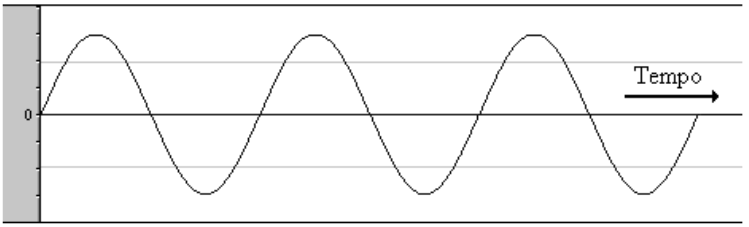
\includegraphics[scale=0.4]{figuras/ondaSenoidal.png}
   Fonte: \cite{miletto2004}.
\end{figure}

\citeonline{miletto2004} apresentam os quatro elementos básicos do som, que são:
\begin{enumerate}
\item Altura tonal \newline
Quando se toca as teclas de um piano, nota-se que os sons são mais agudos quanto mais tocados à direita e mais graves quanto mais se tocar à esquerda. Essa “altura” de um som, ou seja, se é alto ou baixo, agudo ou grave, é chamada “altura tonal”.

Uma repetição de uma onda periódica é chamada de ciclo. Quando são comparados em um osciloscópio sons com alturas tonais diferentes, nota-se que difere o número de ciclos por unidade de tempo. Quanto mais agudo o som, maior o número de ciclos por unidade de tempo e quanto mais grave o som, menor será este número. O número de ciclos dentro do intervalo de um segundo é geralmente chamado freqüência e expresso em unidades chamadas hertz (Hz). 100Hz indica que a vibração ocorre com uma freqüência de 100 ciclos por segundo. Quanto maior o valor em hertz, mais agudo é o som. Dobrando a freqüência de um som, este é elevado em uma oitava, então é possível dizer que a freqüência e a altura tonal estão relacionadas logaritmicamente. A faixa de freqüências que podem ser ouvidas por um ouvido humano é de aproximadamente 20Hz para os sons mais graves e de até 20.000Hz para os sons mais agudos.

\item Volume \newline
Se uma tecla de piano é pulsada fortemente, o som produzido será forte. Se for pulsada suavemente, o som produzido será fraco. As denominações alto e baixo devem ser utilizadas de maneira correta apenas para designar a altura tonal e não o volume. Através de um osciloscópio, a mudança no volume de um som pode ser vista como uma diferença na altura das ondas. A altura de uma onda chama-se “amplitude”. Quanto maior a amplitude, mais forte é o som. Portanto o volume de um som é determinado pela amplitude (altura da onda). Ao contrário do que é falado coloquialmente, um som alto, do ponto de vista da amplitude corresponde a um som forte. Já um som baixo, corresponde a um som fraco.

\item Timbre \newline
Um clarinete e uma flauta não produzem o mesmo som ao serem tocados com a mesma altura tonal e o mesmo volume. Isso se deve ao fato de haver um fator distinto a mais para o som além da altura tonal e do volume. Este fator é o timbre. Observando-se sons com timbres diferentes, através de um osciloscópio, nota-se que as formas de onda diferem entre si. De um modo geral, formas de ondas arredondadas produzem um timbre mais suave enquanto que as formas de ondas ponteagudas dão um timbre mais penetrante e estridente.

Na Figura \ref{fig:ondaTimbre} são mostradas três formas de onda básicas, seus timbres característicos e os instrumentos que se assemelham a cada caso.

\begin{figure}[!htb]
   \centering
   \caption{Formas de onda simples e seus timbres}\label{fig:ondaTimbre} 
   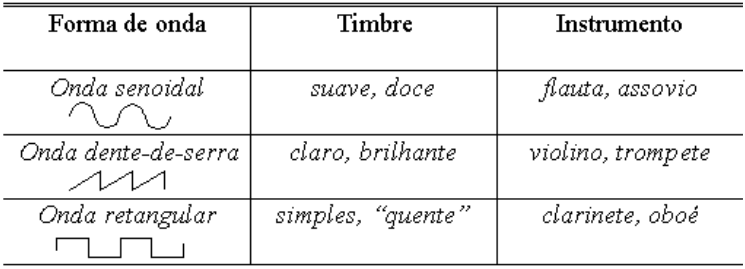
\includegraphics[scale=0.4]{figuras/ondaTimbre.png}
   Fonte: \cite{miletto2004}.
\end{figure}

\item Envolvente da Onda \newline
Trata-se da variação do som em um transcurso de tempo. Mais precisamente, a variação de cada um dos três elementos em um transcurso de tempo que vai desde o começo do som até um ponto do tempo onde ele desaparece completamente. Se um violino for tocado com arco, por exemplo, geralmente o volume do som aumenta gradualmente e também o timbre e a altura tonal mudam ligeiramente. Estas mudanças no tempo são o que determina o timbre característico de um violino, além do seu espectro harmônico. Por outro lado, o relaxamento do som de um piano é um caimento contínuo. Sem este caimento seria muito difícil distingüi-lo do som de uma flauta. Envolventes são, portanto, as mudanças de altura tonal, volume e timbre em um transcurso de tempo. Ocasionalmente, a mudança apenas do volume (amplitude) em um transcurso de tempo é também chamada envolvente.
\end{enumerate}

Segundo \citeonline{miletto2004} é possível encontrar dois tipos de sons: Sons Complexos e Sons Harmônicos ou Parciais.

Os sons complexos são formados por ondas simples (ondas senoidais) que são os harmônicos e a fundamental. Os harmônicos ou parciais são múltiplos da freqüência básica ou fundamental. A fundamental de um som complexo é o componente de mais baixa freqüência. A freqüência fundamental e seus harmônicos constituem a série harmônica. A resultante é uma forma de onda que representa um som complexo.

E o som é dividido em sons musicais e não-musicais dependendo do tipo de vibração principal. Os sons com vibrações regulares (ou seja, sons em que existem muito poucos componentes distintos dos harmônicos) são considerados musicais, enquanto os sons causados por vibrações irregulares complicadas (ou seja, sons com muitos componentes que não são harmônicos), cuja altura tonal não pode, portanto, ser medida, são chamados sons não-musicais. Os sons não-musicais incluem também os sons do tipo desagradáveis. A maioria dos sons usados na música são, por pressuposto, sons musicais. Várias classes de ruídos, como os produzidos por instrumentos de percussão, são também usados para realizar o efeito musical.

\section{Informação Musical}
Para \citeonline{miletto2004} o processo de representar numericamente o som é chamado de digitalização. Um som contendo freqüências limitadas pode então ser representado por uma seqüência de simbolos quantificados ou quantificáveis, ou seja, de números. Segundo \citeonline{setzer2001} , dado é uma sequencia de números, portanto, um texto, fotos, figuras, sons gravados e animação são dados, pois todos podem ser quantificados. Um dado é necessariamente uma entidade matemática e, desta forma, é puramente sintático. Isto significa que os dados podem ser totalmente descritos através de respresentações formais, estruturais e obviamente ser armazenados em um computador e processados por ele. O processamento de dados em um computador limita-se exclusivamente a manipulações estruturais dos mesmos, e é feito por meio de programas. Estes são sempre funções matemáticas, e portanto também são "dados". Exemplos dessas manipulações nos casos de textos são a comparação com outros textos, etc.

Sendo o dado puramente sintático, ao incluir um “significado” implícito na palavra, usado para sua caracterização, é gerado a informação, que é necessariamente semântica.

O autor expõe que a informação é uma abstração informal (isto é, não pode ser formalizada através de uma teoria lógica ou matemática) que está na mente de alguém, representando algo significativo para essa pessoa. Utilizando-se da frase “Paris é uma cidade fascinante” é um exemplo de informação – desde que seja lida ou ouvida por alguém, desde que "Paris" signifique para essa pessoa a capital da França (supondo-se que o autor da frase queria referir-se a essa cidade) e "fascinante" tenha a qualidade usual e intuitiva associada com essa palavra.

A informação pode ser armazenada em um computador, ou melhor, a sua representação em forma de dados e não a informação propriamente dita. Essa representação pode ser transformada pela máquina, como na formatação de um texto (o que seria uma transformação sintática), mas não pode mudar o significado, já que ele depende de uma pessoa que possui a informação. Os dados são sempre incorporados por alguém como informação, porque os seres humanos buscam constantemente por significação e entendimento \citeonline{setzer2001}.

Á partir daí, a autora \citeonline{barros2012} expõe que um dado musical é resultado de um processo de significação social. Assim, a música é uma expressão humana construída socialmente e objetivada por meio de sua comunicação oral, registro sonoro ou representação gráfica.

Para \citeonline{almeida2007}, a obra musical é efêmera e abstrata, pois só se concretiza no momento de cada interpretação, na execução da música. \citeonline{berger&luckmann2014} afirmam que:

\begin{citacao}
A expressividade humana é capaz de objetivações, isto é, manifesta-se em produtos da atividade humana que estão ao dispor tanto dos produtores quanto dos outros homens, como elementos que são de um mundo comum.
\end{citacao}

Para \citeonline{angeles2010,pinheiro&loureito1995} a informação é o que se acrescenta a uma representação. Segundo o autor, recebemos informação se o que conhecemos é alterado. Informação é o que logicamente justifica alteração ou reforço de uma representação ou de um estado de coisas. As representações podem ser explícitas (como em um mapa, ou em uma proposição), ou podem estar implícitas no estado de atividade dirigida do receptor.

A informação musical apresenta determinadas especificidades de comportamento na sua produção, objetivação e uso, pois a manifestação da música apresenta-se carregada de características próprias. \citeonline{michels1992} explica que a música contém dois elementos: o material acústico e a ideia intelectual, sendo que tais elementos não se encontram justapostos, mas sim, se combinam para formar uma imagem unitária. Portanto, a compreensão completa da música está diretamente ligada com o reconhecimento do contexto histórico e social de sua origem, com a interpretação pessoal e individual do ouvinte, e com os aspectos sonoros que a constituem, dessa forma, a música tem diferente significações para cada indivíduo.

\citeonline{lima&santini2006} afirmam que:

\begin{citacao}
A música é um produto social e simbólico de grande importância nas diferentes formações culturais, principalmente se considerarmos a sua capacidade de criar vínculos afetivos e cognitivos entre as pessoas.
\end{citacao}

A compreensão da música como informação é ainda bastante recente. O estudo mais significativo e considerado, dentro da literatura especializada, como pioneiro na conceituação e estudo da música como fonte de informação é o de Alexander McLane. Em 1996 o autor publicou em um capítulo do ARIST \abreviatura{ARIST}{Annual Review of Information Science and Technology} o artigo intitulado \textit{Music as Information} onde formaliza a música como informação.

\section{Armazenamento da Informação Musical}

Até o surgimento dos inventos tecnológicos, a música era um meio de comunicação exclusivamente presencial. Apesar das formas de registros, a exemplo das partituras, possibilitarem a execução de uma obra em diferentes momentos e lugares, a reprodução do que ali estava representando nunca seria a mesma. Com o decorrer do tempo as técnicas e invenções aplicadas ao processo de gravação do som foram surgindo e se aperfeiçoando, resultando em aparelhos reprodutores e suportes cada vez mais versáteis e manipuláveis \cite{daquino2012}. Especialmente após o desenvolvimento das coleções em rede na web, com formatos de arquivos compactados e custos decrescentes de armazenamento de arquivos na forma digital, a música se tornou um objeto de consumo universal e extremamente acessível \cite{gomes2015}.

O primeiro invento significativo para o armazenamento de músicas foi o fonógrafo, patenteado por Thomas Edison em 1877. Inicialmente cilindros feitos de folha de estanho e mais tarde substituídas por metal ou cera. Apesar do enorme passo na evolução do armazenamento musical, o fonógrafo era um aparelho bastante limitado. O aparelho permitia a gravação e reprodução sonora, mas não possibilitava a realização de cópias \cite{marchi2005}.

Dez anos mais tarde, em 1887, surgiu o gramofone, considerado o sucessor direto do fonógrafo. A diferença entre as duas tecnologias é que usava discos planos de cera, vinil, cobre e goma laca em vez de cilindros. Tendo uma capacidade maior de armazenamento e reprodução das músicas.

Dentre as invenções mais importantes para o armazenamento e a reprodução sonora está o disco de vinil, lançado em 1948, comumente conhecido como long-play (LP). Era um disco com rotação por minuto mais demorada, o que permitia aumentar a capacidade de armazenamento da informação na superficie do vinil \cite{marchi2005}.

Cartucho 8-track, foi popular nos EUA entre as décadas de 60 e 70, mas lançado para uso comercial em 1958. Foi a pioneira em armazenar dados musicais em fitas magnéticas, técnica que mais tarde originou outros mecanismos de armazenamento como os HDDs.

Em 1963, com a evolução dos cartuchos 8-track, foi o lançamento da fita cassete ou compact cassette. Com a vantagem de serem menores, sugiram novas possibilidades de comércio e consumo de gravações sonoras. Além da portabilidade e praticidade da fita, surgiu com ela a possibilidade de realização de cópias e edições \cite{marchi2005}.

A paritr da década de 1980 com a intensificação do uso de \textit{hardwares} e \textit{softwares}, já eram notáveis o aperfeiçoamento e disseminação de programas informáticos específicos e o barateamento da tecnologia digital. Neste contexto surge o Compact-Disc (CD \abreviatura{CD}{Compact-Disc}), comercializado a partir de 1982, acabou por se tornar um dos meios de armazenamento de dados musicais mais populares das décadas seguintes, principalmente de música comercializada, sendo o principal representante do desenvolvimento da indústria fonográfica, com produção em massa e padronizada. Além de quebrar paradigmas na época, o CD foi inspiração para o desenvolvimento de outros meios de armazenamento como os DVDs e os discos de Blu-ray.

Entre 1990 e 1992, surgiram os miniCDs e miniDiscs, discos menores e com capacidade de armazenamento reduzida, com o intuito de substituir os CDs, mas a ideia não vingou e foi pouco usado. Apesar da capacidade, apenas o miniDisc teve grande sucesso no Japão \cite{marchi2005}.

O MP3 Player revolucionou a forma como as músicas eram armazenadas e ouvidas no ano de 1998. Ele praticamente liquidou com todas as tecnologias antecessoras por ser facilmente transportado em qualquer bolso ou mochila e pela sua longa vida útil, além do aumento gradativo de armazenamento com o passar dos anos.

No ano de 2000, com a popularização de eletrônicos com portas USB, como computadores, televisores e aparelhos de som – inclusive automotivos, deu aos pendrives mais uma utilidade: a de armazenamento de músicas. Inicialmente oferecido com míseros 8MB de armazenamento disponível. Possuindo atualmente modelos muito mais velozes e “espaçosos”.

Em 2005, surge os cartões de memória microSD, inicialmente usados em celulares, mas seu enorme espaço de armazenamento logo foi adotado por outros tipos de aparelhos eletrônicos \cite{marchi2005}.

O streaming tomou forma no final da década de 80 e começou a se desenvolver na década de 90, com a evolução dos SGBDs \abreviatura{SGBD}{Sistemas de Gerenciamento de Banco de Dados} e o surgimento do Banco de Dados Orientado a Objetos (BDOO \abreviatura{BDOO}{Banco de Dados Orientado a Objetos}) \cite{junior&segundo2008}, que possibilitou o armazenamento de multimidias e a primeira rádio online surgiu em 1994. Porém, a infraestrutura precária e baixa disseminação da internet nesse período, fez com que se popularizasse á partir de 2008, possuindo coleções de músicas amplamente disponíveis na internet. Assim como a popularização de aplicativos móveis, conhecido normalmente por app, que oferecem mais de 30 milhões de música a seus usuários, por exemplo, "Spotify"\footnote{https://www.spotify.com/br/} e "Deezer"\footnote{https://www.deezer.com/br/}.O MP3 Player revolucionou a forma como as músicas eram armazenadas e ouvidas no ano de 1998. Ele praticamente liquidou com todas as tecnologias antecessoras por ser facilmente transportado em qualquer bolso ou mochila e pela sua longa vida útil, além do aumento gradativo de armazenamento com o passar dos anos.

Entretanto, os tradicionais métodos de representação e recuperação de informação, que se baseiam na linguagem natural ou controlada — em documentos-texto completos ou metadados — tem seu foco voltado para “ambientes de palavras”. Sendo assim, os documentos são traduzidos em palavras para representação simbólica das ideias neles contidos, e os mecanismos de busca desenhados para recuperá-los têm sua construção baseada em definições, sinônimos, e as mais variadas relações entre palavras \cite{lima&santini2006}.

E a recuperação dessa informação pode continuar a funcionar em “ambientes de palavras” ou tradicionais, porém só será bem sucedida se esses documentos multimídias puderem ser representados de acordo com as suas peculiaridades.

\section{Representação e Estruturas da Informação Musical}

Criaram-se muitas formas de codificar o som para que seja processado em computadores, o que resulta na existência de uma quantidade equivalente de formatos de arquivo para o armazenamento do som digitalizado. Os formatos de arquivo mais utilizados para o processamento de som são:

\begin{itemize}
   \item Wave, da Microsoft (extensão .wav);
   \item AIFF, da Apple (extensão .aiff ou .aif);
   \item Sun Audio, da Sun (extensão .au);
   \item Real Audio, da RealNetworks (extensão .ra);
   \item MPEG Layer 3 (extensão .mp3);
   \item Windows Media Audio, da Microsoft (extensão .wma).
 \end{itemize}
 
 Os formatos Wave e AIFF são do tipo áudio digitalizado sem compressão. Baseiam-se na codificação PCM (Pulse Code Modulation), onde a própria onda sonora é representada como uma sucessão de números correspondentes às amplitudes do sinal medidas a uma freqüência constante. Esse tipo de codificação origina normalmente um grande volume de dados, na ordem de 0,6 MB a 10 MB por minuto de gravação, dependendo da qualidade definida para o arquivo. Por conseqüência, exige muito espaço para seu armazenamento definitivo. Sua única vantagem é a reprodução fiel do áudio, se o arquivo for gravado com qualidade de CD.

Uma das alternativas é a compressão desse tipo de arquivos, reduzindo o seu tamanho. Diferentes técnicas desenvolvidas acabaram por originar novos formatos de arquivos, como o Sun Audio (que também é aceito pela plataforma Apple), o MPEG-3, o Real Audio e o Windows Media Audio. Esses são, portanto, formatos de arquivos tipo áudio digitalizado com compressão.

Alguns desses algoritmos são muito eficientes, alcançando taxas de compressão de até 12:1 se for mantida uma aparente qualidade, no caso do MPEG-3 (ou até maiores, mas com declínio na qualidade). Ou seja, o arquivo não comprimido poderá ser reduzido a 1/12 do seu tamanho original. O problema é que essas taxas só são alcançadas através de compressão com perdas: parte da informação sonora é descartada, o que reduz a fidelidade da representação em relação ao áudio original.

Outro problema dos arquivos do tipo áudio digitalizado, além do grande volume de dados gerado, é que eles representam a informação sonora porém nenhuma informação musical. Isso quer dizer que, se quisermos manipular os sons no nível de elementos musicais, para alterar parâmetros da música ou gerar uma música nota por nota, por exemplo, teremos que buscar uma representação mais adequada a esse objetivo.

Felizmente essa opção existe e é adotada na codificação MIDI. Essa codificação é uma representação da informação musical. Em geral, arquivos MIDI (extensão .mid ou .smf) contém o equivalente a uma partitura para o computador, mais especificamente para o sintetizador presente na placa de som. Seu código são instruções para um sintetizador, correspondentes a eventos musicais como soar uma nota, silenciar uma nota, mudar o andamento ou o tom da música, etc. O sintetizador, por sua vez, interpreta este código e o executa, podendo usar vários timbres de instrumentos simultaneamente. O tamanho desses arquivos, portanto, tende a ser bem reduzido, já que a codificação de
eventos musicais pode ser bem compacta. A limitação desse sistema está, justamente, no sintetizador, pois de sua qualidade dependerá a qualidade final da música executada. Isso também quer dizer que a mesma música poderá soar bastante diferente se tocada em diferentes sintetizadores.

MIDI é a sigla de Musical Instrument Digital Interface, um padrão de comunicação de dados criado em 1983 por um acordo entre diversos fabricantes de instrumentos musicais norte-americanos e japoneses, para possibilitar a transferência de informações entre instrumentos musicais e computadores.

O padrão MIDI usa tecnologia digital, codificando eventos musicais em dados binários (bits) que são transferidos por meio de uma linha física (cabo MIDI) de um equipamento para outro. Todos os detalhes técnicos relativos aos códigos e os circuitos básicos necessários à comunicação MIDI são definidos na MIDI Specification 1.0, publicada pela MIDI Manufacturers Association (MMA, antiga International MIDI Association) (MIDI MANUFACTURERS ASSOCIATION , 2004; M C Q UEER , 1989).

Embora o objetivo principal do MIDI seja transferir informações de caráter musical, tais como a execução de notas e outros controles de expressão, seu uso tem sido expandido de tal forma que atualmente o MIDI é usado não só para a transferência de dados relativos à execução musical propriamente dita, mas também para outras aplicações de alguma forma correlatas à música, como controle de iluminação e equipamentos de áudio.

Na forma mais simples de se usar MIDI, um músico pode controlar um teclado a partir de outro (controle remoto), pois todas as suas ações de execução musical são codificadas e transmitidas pelo cabo MIDI para o outro teclado, que recebe, decodifica e executa aquelas mesmas ações. Assim, numa implementação bastante simples, é possível tocar dois ou mais instrumentos a partir de um deles, o que possibilita, entre outras coisas, a superposição dos sons dos vários instrumentos controlados simultaneamente.

É importante frisar que as informações MIDI transferidas de um equipamento (mestre) para outros (escravos) não carregam consigo nenhum sinal de áudio (som). Essas informações são mensagens que codificam as ações do músico, tais como o ato de pressionar uma tecla, ou o de soltar uma tecla. O som (áudio) conseqüente do ato de pressionar uma tecla não é transferido via MIDI, mas sim gerado em cada um dos instrumentos da cadeia. Dessa forma, quando um instrumento “mestre” comanda outro via MIDI, basicamente ele “diz” ao outro quais as notas que devem ser tocadas, mas o som (áudio) do segundo instrumento será determinado pelo próprio “escravo”.

Principais características do sistema MIDI

\begin{itemize}
    \item Sistema digital de comunicação de dados.
    \item Transmissão serial assíncrona.
    \item Taxa de transmissão: 31.250 bits/s.
    \item Comunicação unilateral.
    \item Permite padronizar a comunicação entre os instrumentos (protocolo MIDI).
    \item Facilita a ligação entre instrumentos e computadores.
    \item Permite a edição de qualquer evento musical através de software.
    \item Permite tocar vários instrumentos simultaneamente.
    \item Permite gerar arquivos MIDI Standard.
\end{itemize}

\section{Recuperação da Informação Musical}

A área de pesquisa denominada Music Information Retrieval(MIR) ou Recuperação da Informação Musical (RIM), tradução literal incorporada pela corrente da área no Brasil. Porém, como apontado por \citeonline{santini&souza2007} a produção de pesquisas voltadas para a área são praticamente inexistentes na literatura nacional.

De acordo com \citeonline{futrelle&downie2002} a Recuperação da Informação Musical é:

\begin{citacao}
[...] uma agenda de pesquisa que, de forma geral, pretende desenvolver formas de gestão de coleções de obras musicais para preservação, busca, acesso e outros usos.
\end{citacao}

A agenda de pesquisas sobre a RIM intensificou sua produção recentemente com a explosão do interesse em coleções em rede que contenham obras musicais na forma digital, possibilitadas pelo desenvolvimento das citadas técnicas de compressão de áudio. Os pesquisadores de RIM observam que a motivação maior para essa área de pesquisa é o grande volume de música digital disponível na Internet que quanto mais cresce menos possibilita sua recuperação eficiente visto que estão apenas disponíveis aos montes, mas sem o tratamento adequado \cite{gomes2015}.

A área de RIM conta com profissionais das mais diversas áreas inclusas na questão do tratamento e recuperação da informação musical como apresentado na tabela a seguir, traduzida por \citeonline[p.11]{santini&souza2007}

\begin{figure}[!htb]
   \centering
   \caption{Comunidades de RIM}\label{fig:comunidadeRim} 
   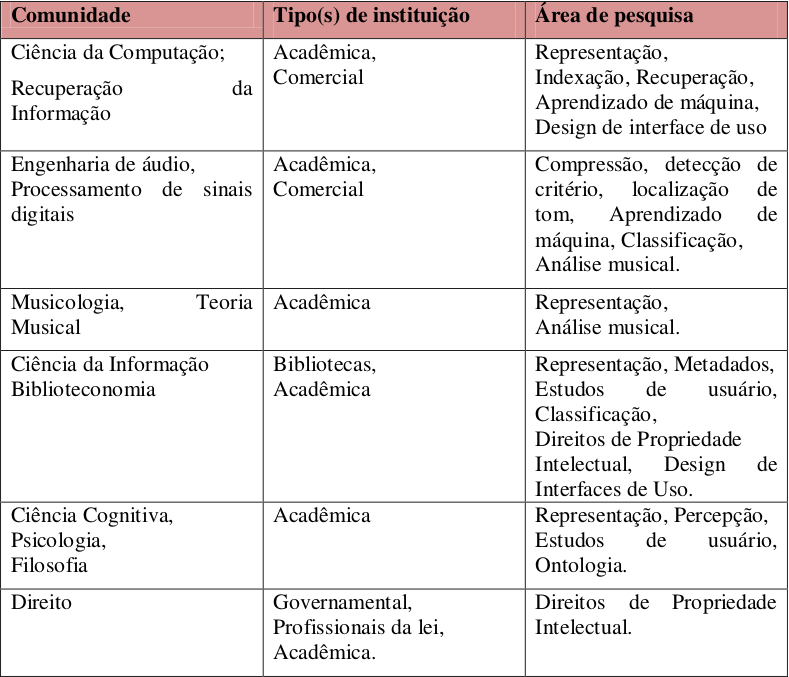
\includegraphics[scale=0.4]{figuras/comunidadeRim.png}
   Fonte: \cite{futrelle&downie2002}.
\end{figure}

A origem de RIM não apresenta uma ação interdisciplinar, o que prejudica todo o seu processo de comunicação científica. Como pontua \citeonline[p.11]{santini&souza2007}:

\begin{citacao}
(...) não há uma sociedade (inter)disciplinar de RIM; um periódico ou livro-texto fundador onde pessoas interessadas podem adquirir as bases teóricas e práticas de RIM. Com exceção de alguns pequenos encontros interdisciplinares, muitos pesquisadores estão apresentando seus resultados para membros das suas próprias disciplinas. A literatura de RIM é difícil de ser localizada, lida e estudada, o que dificulta construir e sustentar uma área de pesquisa respeitável, próspera.
\end{citacao}

A escassa produção científica a respeito do tema e as características impostas pelas músicas acarretam em certas dificuldades para sua representação.

Como elucidado no final do item 2.1 desta seção, o ponto de partida para os estudos sobre a música como fonte de informação e tratamento, representação e recuperação foi dado em 1996 por Alexander McLane. Neste mesmo período já era possível identificar o desenvolvimento de tecnologias de compressão de arquivos digitais de música para transmissão na Internet e a popularização da Internet no mundo \cite{santini&souza2007}.

Em seu estudo McLane direciona sua discussão para os grandes problemas relacionados à representação de documentos de música e à recuperação destes documentos. McLane analisa aspectos significantes da música – sua notação e seu som – e propõe algumas ideias para sistemas de recuperação de música, e formaliza a música como informação segundo três visões: visão subjetiva, visão objetiva e visão interpretativa. Segundo o autor, as necessidades dos vários tipos de análises musicais são tão diversas que é preferível considerar três “visões” sobre a representação da obra musical.

Em resumo adaptado, \citeonline{santini&souza2007} apresenta as principais características das visões estabelecidas por \citeonline{mclane1996}.

\begin{itemize}
    \item A visão \textbf{subjetiva} da informação musical se faz por meio do uso do esquema de notação para representação da informação musical. A subjetividade se dá porque a escolha de elementos de notação geralmente representa uma obra em “contexto-dependente” sendo assim a decisão da notação pode incluir ou excluir aspectos particulares da obra.
    \item A visão \textbf{objetiva} está vinculada a audição e ao momento da execução musical. Um som gravado pode ser identificado como visão objetiva da obra musical. A sonoridade se caracteriza como objetiva por não se configurar como uma representação, mas como a obra em sua essência. O som musical uma vez gravado torna-se fixo e não está mais sujeito a variações editoriais e de performance. Segundo McLane esta visão pode ser considerada a mais completa representação da música, ao passo em que inclui as facetas: tom, tempo, harmonia, editorial e timbre.
    \item A visão \textbf{interpretativa} é realizada através da análise de alguns aspectos da obra, engloba informações que não são diretamente dependentes do documento. Entram nessa categoria classificações e esquemas analíticos que elucidam características como o gênero musical e avaliações críticas.
\end{itemize}

De acordo com \citeonline[p.11]{cruz2014}:

\begin{citacao}
Dentre as visões propostas por McLane (1996), a interpretativa possui uma característica interessante porque permite a independência formal do documento musical em relação ao suporte que o contém, assim como foi possível na informação textual.
\end{citacao}

Segundo \citeonline[p.5]{mclane1996,santini&souza2007}, a representação da informação musical pode abranger as três visões apresentadas dependendo das necessidades de informação da comunidade usuária. De acordo com tradução das autoras, a conclusão de McLane seria a de que:

\begin{citacao}
Ambas as escolhas sobre a visão da representação da música e o grau de complementação da representação de uma obra depende da necessidade de informação do usuário. A recuperação de informação é um processo interativo que depende do conhecimento do usuário e do nível de complexidade da informação desejada. No caso da necessidade da simples identificação de uma obra musical, onde a informação bibliográfica não é unicamente suficiente, pode-se limitar a uma visão subjetiva envolvendo um subconjunto relativamente pequeno de elementos notados de uma obra, frequentemente o tom inicial de uma frase melódica. A representação tonal pode ser de forma tal que provavelmente o usuário espera e está apto para formular a indagação usando a mesma terminologia, ou pelo menos uma que é traduzível na forma de representação.
\end{citacao}

Sendo assim, percebe-se que a recuperação da informação da música depende tanto da complexidade e da forma como a informação é representada como do nível de conhecimento prévio do usuário. Para \citeonline[p.5]{santini&souza2007}: “Quanto menor o conhecimento do usuário, maior a necessidade de diferentes formas de representação. Cada visão da representação da música, demonstrada por McLane, não é suficiente isoladamente para identificar uma obra.”.

Outro autor presente nos estudos relacionados à representação e recuperação de informação musical e um dos representantes da área de RIM é o professor J. Stephen Downie da Universidade de Illinois, nos Estados Unidos. Downie escreveu, em 2003, outro artigo tido como marco no estudo da informação musical, intitulado Music Information Retrieval também em um capítulo do ARIST. No trabalho em questão, \citeonline{downie2003} examina a multidisciplinaridade da área de RIM, identifica e explica alguns problemas relacionados a questão da representação e recuperação da informação musical. Para isso \citeonline{downie2003} resume a questão em quatro grandes desafios a serem enfrentados pelos pesquisadores da área.

De acordo com \citeonline[p.5]{downie2003,santini&souza2007} os quatro desafios seriam:

\begin{citacao}
    \begin{enumerate}
        \item Considerar permanentemente as diferentes formas de representação da música, o que caracteriza o “desafio multirepresentacional”. O copyright faz parte deste desafio.
        \item Cada época histórica e cada formação cultural criam modos próprios e singulares de se expressar através da música. A música transcende as fronteiras culturais e temporais. A ampla variedade de expressões musicais coloca em evidência o “desafio multicultural”.
        \item Compreender e responder às diferentes formas de interação individual com a música e com os siste mas de RIM constitui o “desafio multiexperimental”.
        \item Maximizar os benefícios de ter uma comunidade multidisciplinar de pesquisadores, enquanto minimiza a desvantagem inerente, representa o “desafio multidisciplinar”.
    \end{enumerate}
\end{citacao}

O desafio multirepresentacional é dividido em sete facetas a serem consideradas na descrição da música e que representam a estrutura musical \cite{downie2003}. São elas: tonal, temporal, harmônica, de timbre, editorial, textual e faceta bibliográfica. Sendo as quatro primeiras relativas a aspectos sonoros da música com formas gráficas de representação em figuras rítmicas ou notações musicais, enquanto que as três últimas são representadas na forma gráfica e dizem respeito às informações de produção, intérprete, compositor, copyright, data de produção e outras \cite{barros2012}.

Apesar de completas, a interação dessas facetas resulta em um complexo tratamento da informação musical, visto que cada faceta citada possui por si só uma complexidade inerente e sofre um tipo de representação enquanto produto. As autoras \citeonline[p.8]{santini&souza2007} resumem a problemática multirepresentacional da seguinte forma:

\begin{citacao}
    A complexa interação entre as facetas da música - tempo, harmonia, timbre, freqüência, editoria, texto e bibliografia – evidencia um dos principais problemas de RIM: o desafio multirepresentacional. A escolha da representação da música – se baseada em símbolos, áudio ou ambos – adiciona-se a diversas questões: como, por exemplo, cada escolha determina a tecnologia, a organização, a recuperação e a interface entre requisitos e capacidades dos sistemas.
\end{citacao}

Sendo assim, apesar de possuir as facetas estabelecidas pelo autor, a estrutura da música incorpora elementos extras que nos permitem defini-la como um objeto informacional mais complexo. Além das facetas definidas por  \citeonline[p.283]{downie2003,cruz2014}, a estrutura musical:

\begin{citacao}
    [...] incorpora elementos adicionais que permitem defini-la como um objeto informacional musical mais amplo, dotado de conteúdo – atributos internos e metadados descritivos – e, de contexto – associações com outros objetos musicais e não musicais, e com situações ou eventos em que este objeto musical está inserido.
\end{citacao}

O segundo desafio (multicultural) nasce da condição inerente à música de ser uma objetivação de algo extremamente subjetivo: a expressão humana. Sendo assim, sofre a interferência de uma grande variedade de fatores, da cultura vigente no momento da produção musical e da localização geográfica desta produção.

O desafio multiexperimental diz respeito à percepção da música como experiência individual ou coletiva capaz de causar diferentes reações em diferentes momentos e situações, de cada mente e humor individual. Neste caso ouvir uma música gravada funciona como “ajuda memória” que traz a tona experiências prazerosas ou dolorosas relacionadas a uma música em especial (DOWNIE, 2003 apud SANTINI; SOUZA, 2007, p. 9). As variações de pessoa para pessoa na forma de apropriação, apreciação e nos tipos de experiências emocionais que a música evoca demonstram de maneira pragmática o desafio multiexperimental.

O quarto e último desafio estabelecido por Downie (2003) é o desafio multidisciplinar. Como citado anteriormente, a diversidade intelectual da comunidade de pesquisadores de RIM é, ao mesmo tempo, uma vantagem e uma adversidade. A heterogeneidade das visões de mundo das disciplinas apresenta um problema particular. Cada disciplina traz suas crenças, práticas, questões de pesquisa e paradigmas de avaliação (DOWNIE, 2003). De acordo com Futrelle e Downie (2002), não há uma aceitação comum dos objetivos, técnicas e resultados obtidos nas pesquisas referentes à informação musical.

Percebe-se por tanto, que se por um lado, a ação multidisciplinar dos pesquisadores envolvidos com o tema possibilita o surgimento de diversos avanços tecnológicos e que a cada dia são divulgadas novas soluções para o tratamento de conteúdos musicais, com algoritmos mais sofisticados, novas formas de indexação de músicas, novos tipos de interfaces de áudio e novas formas de representação musical, em contrapartida, é notável a dificuldade de comunicação entre esses resultados. Nota-se ainda a dificuldade de identificação desses conteúdos musicais, porque a música é complexa e possui um leque de propriedades que possibilitam abordagens, às vezes, contraditórias (CRUZ, 2008).

A análise documental da informação musical para sua representação apresenta complexidades, pois exige diferentes técnicas de extração de informações para distintas formas de apresentação.(DOWNIE, 2003).
\chapter{Soluções Existentes} \label{solucoes}
Nos últimos anos, várias plataformas digitais de \textit{streaming} têm surgido, derivado das intensas procuras pelo usuário por música online. Com a variedade de serviços que temos ao nosso dispor, este capítulo apresenta de forma resumida algumas soluções existentes para busca de dados musicais, de forma comercial e acadêmica, com base nos seus sites oficiais.

%%COMERCIAL%%
\section{Comercial}

%MUSICID%
\subsection{MusicID}
\textit{Gracenote Inc.} foi fundada em 1998, é uma empresa que fornece metadados de música, vídeo e esportes e tecnologias de reconhecimento automático de conteúdo para empresas e serviços de entretenimento em todo o mundo.

Segundo o site da companhia\footnote{http://www.gracenote.com/music/music-recognition/}, tradução nossa:

\begin{citacao}
O Gracenote MusicID\textregistered é o padrão para reconhecimento de música. Ele ajuda os fãs a desbloquear seus álbuns e faixas favoritos na nuvem e a descobrir novas músicas com seus celulares, além de permitir o monitoramento de músicas para detentores de direitos e profissionais do setor \cite{musicid1998}.
\end{citacao}

O Gracenote MusicID\textregistered, faz o reconhecimento de músicas que são tocadas ao seu redor, combinado ao uso de \textit{fingerprints} e correspondência de texto para identificar arquivos de música digital a um banco de dados mundial de informações musicais. Uma vez reconhecidos, os arquivos são organizados por nome de faixa, nome do álbum e caminhos de pastas para garantir que as músicas e os álbuns certos sejam sempre correspondidos.

%SHAZAM%
\subsection{Shazam}
\textit{Shazam Entertainment Ltd.} foi fundado em 2000 com a idéia de prover um serviço que pudesse conectar as pessoas à musica, permitindo a identificação da música através dos \textit{Smartphones}.

A aplicação usa o microfone do \textit{Smartphone} ou do computador para capturar uma pequena amostra de música, e então, realiza a identificação da música em um grande banco de dados com mais de 12 bilhões de músicas e, além disso, deve ter um baixo número de erros, ao mesmo tempo que tem uma alta taxa de acertos.

Segundo o site da companhia \footnote{https://www.shazam.com/pt/company}:

\begin{citacao}
Shazam é uma aplicação móvel que reconhece música e conteúdos de TV à sua volta. É a melhor maneira de descobrir, explorar e compartilhar a música e os conteúdos de TV que você mais gosta. Levamos 10 anos para alcançar 1 bilhão de tags, 10 meses para chegar a 2 bilhões, 3 meses para ir de 10 a 12 bilhões... É uma aplicação fantástica, agora disponível nas lojas da Apple e Android. E estamos sempre à procura de novas maneiras de encantar os nossos usuários \cite{shazam2000}.
\end{citacao}

Para o trecho de música capturado pela aplicação é criado uma \textit{fingerprint} ou impressão digital, tradução literal icorporada a palavra. Desta forma, é comparada com todas as outras \textit{fingerprints} derivadas das músicas no banco de dados. Se houver uma correspondência, é enviado informações da música para o usuário, como artista, álbum e título da música.

%SOUNDHOUND%
\subsection{SoundHound}
\textit{SoundHound Inc.} foi fundada em 2005, é uma empresa pioneira em desenvolvimento de aplicações para reconhecimento de voz, compreensão da linguagem natural, reconhecimento de som e tecnologias de busca.

Segundo o site da companhia\footnote{https://soundhound.com/about}, tradução nossa:

\begin{citacao}
Acreditamos em permitir que humanos interajam com as coisas ao seu redor da mesma forma como interagimos entre nós: falando naturalmente com telefones celulares, carros, TVs, caixas de música, máquinas de café, e todas as outras partes emergentes do mundo "conectado". Nosso produto mais recente, Hound, utiliza a nossa tecnologia \textit{Speech-to-Meaning}\texttrademark\ para mostrar uma experiência inovadora com os \textit{Smartphones}. Nosso produto \textit{SoundHound} aplica nossa tecnologia a música, permitindo as pessoas descobrir, explorar e compartilhar música ao seu redor, e até mesmo encontrar o nome daquela música presa em suas cabeças cantando ou cantarolando. E através da plataforma Houndify, capacitamos os desenvolvedores para fazerem parte dessa revolução \textit{speech-to-meaning} \cite{soundhound2005}.
\end{citacao}

É através da plataforma independente de Inteligência Artificial Houndify, combinado ao \textit{Automatic Speech Recognition} (ASR) e o \textit{Natural Language Understanding} (NLU) que permite a identificação das músicas de forma rápida e eficiente.

Desta forma, os dois produtos conhecidos no meio musical são:

\begin{enumerate}
    \item SoundHound Music Search \& Play\footnote{https://soundhound.com/soundhound}: É um aplicativo para \textit{Smartphones}, onde é possível descobrir, pesquisar e reproduzir qualquer música com controle de voz. Também é possível pesquisar músicas cantando ou cantarolando, tornando o único app no mundo que pode dar resultados, imediatamente e com precisão, ouvindo você cantar ou cantarolar.
    \item Midomi\footnote{https://www.midomi.com/}: Possui as mesmas características que o item anterior, porém possui versão para \textit{web} e a versão \textit{mobile} é destinado aos modelos mais antigos de \textit{Smartphones}.
\end{enumerate}

%DEEZER%
\subsection{Deezer}
A Deezer nasceu da necessidade de facilitar a vida de seu fundador para ouvir e fazer o \textit{download} de músicas. Com isso, o idealizador da plataforma desenvolveu o \textit{Blogmusik.net} em 2006. Devido a popularidade, houve objeção de detentores de direitos autores, o que gerou o fechamento do site. Pouco tempo depois, um acordo histórico foi assinado e o antigo site voltou ao ar com o nome de Deezer.

Segundo o site da companhia\footnote{https://www.deezer.com/br/company}:

\begin{citacao}
Na Deezer você ouve toda e qualquer música, na hora que quiser. Explore mais de 53 milhões de faixas (e a contagem continua) e descubra artistas e músicas que você vai amar com a recomendação personalizada dos Editores Deezer. A Deezer está em todos os seus dispositivos, tanto online como offline, sem limites de escuta. Música na ponta de seus dedos para todos os momentos do seu dia: amanhecer, ir ao trabalho, relaxar, viver a vida...é só dar play! \cite{deezer2006}
\end{citacao}

A Deezer também conta com uma série de aplicativos que complementam a experiência musical do usuário. O \textit{Stateeztics}, por exemplo, é um in-app exclusivo que traça o perfil musical do usuário e mostra suas estatísticas de consumo a partir do seu histórico sonoro. Outra aplicação disponível é o \textit{Edjing}, que oferece mixagem de músicas com diversas ferramentas de efeitos digitais, além de contar com uma interface bastante intuitiva. Já o usuário que está aprendendo a tocar instrumentos musicais pode contar com o \textit{Chordify}, que reconhece o som que está tocando na Deezer e faz a transcrição automática da harmonia em cifras.

%SPOTIFY%
\subsection{Spotify}
\textit{Spotify Ltd.} foi fundado em 2006, é um serviço de streaming de música, podcast e vídeo, além de ser o mais popular e usado do mundo. A plataforma fornece conteúdo protegido providos de restrição pela gestão de direitos digitais de gravadoras e empresas de mídia. O Spotify é um serviço \textit{freemium}: possui recursos gratuitos com propagandas ou limitações, enquanto recursos adicionais, como qualidade de transmissão aprimorada e \textit{downloads} de música, são oferecidos para assinaturas pagas.

Segundo o site da companhia\footnote{https://www.spotify.com/br/about-us/contact/}:

\begin{citacao}
Com o Spotify, é fácil encontrar a música certa para cada momento – no seu telefone, computador, tablet e outros. Existem milhões de faixas no Spotify. Não importa se você está malhando, em uma festa ou relaxando, a música certa está sempre em suas mãos. Escolha o que quer ouvir ou deixe o Spotify surpreendê-lo. Você também pode navegar pelas coleções de músicas de amigos, artistas e celebridades, ou criar uma estação de rádio e simplesmente aproveitar. Produza a trilha sonora de sua vida com o Spotify. Assine ou ouça de graça \cite{spotify2006}.
\end{citacao}

A plataforma emprega um modelo de distribuição de dados híbrido com uma combinação de compartilhamento de dados ponto-a-ponto (P2P) e uma infraestrutura de servidor. 

O Spotify possui uma \textit{Web API} que permite que desenvolvedores integrem o conteúdo do Spotify em seus próprios aplicativos. O Spotify \textit{Web API} é um serviço com base na arquitetura REST, que retorna em formato JSON os dados sobre álbuns, artistas, faixas, playlists, entre outros. Para acessar outras informações é necessário autenticação OAuth.

%SOUNDCLOUD%
\subsection{SondCloud}
\textit{SoundCloud} foi criado em 2007, é uma plataforma online de publicação de áudio utilizada por profissionais de música. Nele os músicos podem colaborar, compartilhar, promover e distribuir suas composições.
Originalmente, o objetivo do site era permitir que profissionais da música trocassem ideias sobre as composições nas quais estão trabalhando, permitindo uma fácil colaboração e comunicação antes de um lançamento público. Hoje, o site também é utilizado por ouvintes e usuários da web em geral.

Segundo o site da companhia\footnote{https://soundcloud.com/pages/contact}, tradução nossa:

\begin{citacao}
Como a maior plataforma de música e áudio do mundo, o SoundCloud permite que as pessoas descubram e desfrutem da maior seleção de músicas da mais diversificada comunidade de criadores do mundo. Desde o seu lançamento em 2008, a plataforma tornou-se famosa por seu conteúdo e recursos exclusivos, incluindo a capacidade de compartilhar músicas e se conectar diretamente com artistas, bem como descobrir trilhas inovadoras, demonstrações brutas, podcasts e muito mais. Isso é possível graças a uma plataforma aberta que conecta diretamente os criadores e seus fãs em todo o mundo. Os criadores de música e áudio usam o SoundCloud para compartilhar e gerar receita com seu conteúdo com um público global, além de receber estatísticas detalhadas e feedback da comunidade do SoundCloud. Ainda não tem uma conta gratuita? \cite{soundcloud2007}
\end{citacao}

Os usuários registrados podem ouvir o máximo de conteúdo como quiserem e podem fazer o \textit{upload} de até 180 minutos de áudio ao seu perfil. Todos esses recursos são gratuitos e estão disponíveis para todos os usuários registrados do SoundCloud.

A plataforma possui uma API integrada a várias aplicações, que permitem fazer o \textit{upload} ou \textit{download} de música e arquivos de música.

O SoundCloud descreve as faixas de música graficamente como formas de onda e permite aos usuários comentar em partes específicas do áudio (conhecido como comentários cronometrados). Estes comentários são exibidos ao escutar a parte do áudio que estão se referindo. Outras característica inclui reposts, listas de reprodução, seguidores e \textit{downloads} digitais de cortesia.

%MUSIXMATCH%
\subsection{Musixmatch}
\textit{Musixmatch} foi criado em 2010, com o objetivo de mudar a forma como as pessoas experimentam música e letras.

Segundo o site da companhia\footnote{http://about.musixmatch.com/}, tradução nossa:

\begin{citacao}
Musixmatch é a maior plataforma de letras do mundo - onde você pode pesquisar, curtir e compartilhar letras de qualquer música, em qualquer lugar do mundo \cite{musixmatch2010}.
\end{citacao}

A plataforma pode ser acessada através do site e por aplicativo nos \textit{Smartphones}. O Musixmatch digitaliza todas as músicas da biblioteca de música do usuário e encontra letras para todas elas e apresenta a letra conforme a música que estiver sendo tocada. 

Possui também, a capacidade para capturar uma pequena amostra de música (mesma função encontrada em aplicativos como o Shazam e o Soundhound), além de identificar a letra da música e mantê-la sincronizada enquanto a música é tocada.

%ACRCLOUD%
\subsection{ACRCloud}
\textit{ACRCloud} foi criado em 2015, sendo o campeão no campeonato de \textit{Audio Fingerprinting} do MIREX2015, organizado pelo Laboratório Internacional de Avaliação de Sistemas de Recuperação de Informação Musical (IMIRSEL, sigla em inglês).

ACR (\textit{Automatic Content Recognition}) é uma tecnologia de identificação para reconhecimento de conteúdo reproduzido em um dispositivo de mídia. Permitindo que os usuários obtenham rapidamente informações detalhadas sobre o conteúdo que acabaram de experimentar sem qualquer entrada de texto ou esforços de pesquisa.

Segundo o site da companhia\footnote{https://www.acrcloud.com/docs/acrcloud/}, tradução nossa:

\begin{citacao}
O ACRCloud fornece serviços ACR em nuvem para ajudar empresas e desenvolvedores excelentes a criar aplicativos baseados em impressões digitais de áudio, como reconhecimento de áudio (suporte a música, vídeo, anúncios on-line e off-line), monitoramento de transmissão, interatividade de segunda tela, detecção de direitos autorais etc \cite{acrcloud2015}.
\end{citacao}

O ACRCloud é uma plataforma de microseriços na nuvem, que possui reconhecimento de música através de \textit{fingerprints}, além do monitoramento de transmissão com identificação e apresentação de conteúdo, entre outros.

Possui integração com serviços de música como o Spotify, Deezer, entre outros, que permite desenvolvedores acessarem diretamente esses serviços e oferecer links diretos para seus usuários. Também possui o reconhecimento de músicas através do canto.
%https://www.acrcloud.com/pt/music-recognition

%MUSIPEDIA%
\subsection{Musipedia}
%https://www.musipedia.org/about.html
Musipedia é uma enciclopédia aberta de música, criação inspirada no Wikipedia\footnote{https://www.wikipedia.org/}, para localização, edição e expansão de coleções de tons, melodias, e temas musicais.

Os conteúdos podem ser alteradas por qualquer usuário. Um conteúdo pode conter um pedaço de música, um arquivo MIDI, informações textuais sobre o trabalho e o compositor, e o código de Parson (uma descrição aproximada do contorno melódico).

Segundo o site da enciclopédia\footnote{https://www.musipedia.org/about.html}, tradução nossa:

\begin{citacao}
[...]Você pode tocá-lo em um teclado de piano, assobiar para o computador, simplesmente tocar o ritmo no teclado do computador ou usar o código Parsons \cite{musipedia}.
\end{citacao}

A enciclopédia utiliza o mecanismo de pesquisa de melodias \textit{Melodyhound}, onde é possível encontrar e identificar uma música, mesmo que a melodia seja tudo o que você saiba no momento.

%%ACADEMICO%%
\section{Acadêmico}

%MUSIC MINER%
\subsection{MusicMiner} \label{musicminer}
O \textit{Databionic MusicMiner}, desenvolvido como parte de um projeto de pesquisa do Grupo de Pesquisa em Databionics da Universidade de Marburg, na Alemanha, é um navegador para música baseado em técnicas de mineração de dados. Você pode criar \textit{MusicMaps} para visualizar a similaridade de músicas e artistas.

Segundo o site do projeto\footnote{http://musicminer.sourceforge.net/}, é composto pelas seguintes características:

\begin{itemize}
    \item Análise automática de uma árvore de pastas com arquivos de música (MP3, OGG, WMA, M4A, MP2, WAV);
    \item Descrição automática de arquivos de áudio digital por som;
    \item Criação de \textit{MusicMaps} para navegar pelo espaço sonoro com base no paradigma dos mapas geográficos;
    \item Criação visual de \textit{playlists};
    \item Pesquisa de similaridade na coleção de músicas com base no som;
    \item Navegação hierárquica personalizável da base de dados, por ex. gênero/artista/álbum ou ano/artista;
    \item Base de dados flexível, incluindo o armazenamento separado de vários artistas por música, álbuns e listas de reprodução como parte de uma lista de reprodução;
    \item Importação e exportação de meta informações baseadas em XML.
\end{itemize}

O \textit{MusicMiner} é escrito em Java para máxima portabilidade e publicado sob os termos da GPL (General Public License). Tendo como foco principal a pesquisa e o ensino.

Informações mais detalhadas sobre o projeto pode ser consultada em \cite{morchen2005} e \cite{musicminer}.

%YALE%
\subsection{YALE}
Um protótipo para a descoberta de conhecimento deve atender a vários requisitos:

\begin{enumerate}
    \item Deve ser flexível no que diz respeito aos métodos de pré-processamento e análise de dados, ou seja, deve oferecer uma gama muito ampla de métodos diferentes e que a incorporação de novos métodos seja fácil;
    \item Deve ser capaz de processar diferentes tipos de dados de entrada, como séries temporais ou dados de texto, sem esforço adicional para o usuário;
    \item Deve fornecer ampla funcionalidade para avaliação e otimização;
    \item Deve ser fácil de usar, ou seja, não deve exigir que o usuário aprenda um formalismo complexo para o uso.
    
\end{enumerate}

E o sistema Yale\footnote{http://yale.sf.net} foi desenvolvido para atender aos requisitos descritos acima. É um ambiente para experimentos de aprendizado de máquina e mineração de dados que apóiam o paradigma de prototipagem rápida. As aplicações da Yale abrangem tarefas de pesquisa e de mineração de dados do mundo real.

Atualmente, abrange o processamento de texto, áudio, séries temporais e multimídia, simulação de fluxo de dados e tratamento de desvio de conceito, armazenamento em cluster e mineração de dados distribuída.

Como curiosidade, o \textit{MusicMiner}, descrito na subseção \ref{musicminer} extrai os recursos de áudio necessários usando o plugin do sistema Yale.

Informações mais detalhadas sobre o projeto pode ser consultada em \cite{mierswa2006}

%CLAM%
\subsection{CLAM}
CLAM (\textit{C++ Library for Audio and Music})\footnote{http://clam-project.org/} é um \textit{framework}, desenvolvido em C++ no \textit{Music Technology Group} (MTG) na Universidade Pompeu Fabra em Barcelona, Espanha.

O \textit{framework} oferece uma plataforma completa de desenvolvimento e pesquisa para o domínio de áudio e música. Além de oferecer um modelo abstrato para sistemas de áudio, ele também inclui um repositório de algoritmos de processamento e tipos de dados, bem como diversas ferramentas, como entrada/saída de áudio ou MIDI.

O objetivo inicial do projeto CLAM era oferecer uma plataforma C++ de análise/síntese de som completa, flexível e independente de plataforma para atender às necessidades de todos os projetos do MTG. Esses objetivos iniciais mudaram um pouco desde então, principalmente porque a biblioteca não é mais vista como uma ferramenta interna para o MTG, mas como uma estrutura licenciada sob a GPL.

Informações mais detalhadas sobre o projeto pode ser consultada em \cite{amatriain2007}.

%MIR TOOLBOX%
\subsection{MIRtoolbox}
\textit{MIRtoolbox}\footnote{https://www.jyu.fi/hytk/fi/laitokset/mutku/en/research/materials/mirtoolbox} é uma caixa de ferramentas escritas em Matlab, dedicadas à extração de arquivos de áudio de recursos musicais como tonalidade, ritmo, estruturas, etc., desenvolvido pela Universidade de Jyväskylä.

Ele foi projetado especialmente com o objetivo de permitir o cálculo de uma grande variedade de recursos de bancos de dados de arquivos de áudio, que podem ser aplicados a análises estatísticas. Desta forma, poderia ser útil para a comunidade de pesquisa em Recuperação da Informação Musical (MIR), mas também para fins educacionais.

A caixa de ferramentas foi inicialmente concebida no contexto do projeto Brain Tuning financiado pela União Européia (FP6-NEST). Um dos principais objetivos foi investigar a relação entre características musicais e emoção induzida pela música e a atividade neural associada.

A \textit{MIRtoolbox} é oferecida gratuitamente à comunidade de pesquisa, e mais informações mais detalhadas sobre o projeto pode ser consultada em \cite{lartillot2007} e \cite{mirtoolbox}

%AMUSE%
\subsection{AMUSE}
AMUSE (\textit{Advanced Music Explorer})\footnote{https://sourceforge.net/projects/amuse-framework/} é um \textit{framework} licenciado sob a GPL e implementado em JAVA, desenvolvido pela TU Dortmund.

O \textit{framework} fornece diferentes funcionalidades, como: processamento de som convertendo arquivos de áudio MP3 em ondas sonoras; \textit{downsampling} para a conversão de arquivos de áudio mono; escalabilidade usando multi-threading e o gerenciamento eficiente do conjunto de dados que suporta diretamente o formato WEKA ARFF, além de um componente logger integrado. Oferecido gratuitamente à comunidade de pesquisa.

Informações mais detalhadas sobre o projeto pode ser consultada em \cite{vatolkin2010} e \cite{amuse}

%JAVA MIR%
\subsection{Java MIR}
jMIR (Java MIR)\footnote{http://jmir.sourceforge.net/} é um \textit{software} que compõem um conjunto de componentes desenvolvido na CIRMMT e Marianopolis College. Cada um dos componentes pode ser utilizado separadamente ou como um todo.

O software é de código livre implementado em Java para uso nas pesquisas de Recuperação de Informação Musical (MIR). Ele pode ser usado para estudar música na forma de gravações de áudio, codificações simbólicas e transcrições líricas, e também pode extrair informações culturais da Internet. Além de incluir ferramentas para gerenciar e criar perfis de grandes coleções de músicas e para verificar o áudio quanto a erros de produção. É bem documentado e inclui GUIs para aumentar a usabilidade geral.

O objetivo principal do \textit{software} é auxiliar nas pesquisas em classificação automática de música e a análise de similaridade, proporcionando as seguintes características:

\begin{itemize}
    \item Tornar tecnologias sofisticadas de reconhecimento de padrões acessíveis a pesquisadores de música com históricos técnicos e não técnicos;
    \item Eliminar duplicação redundante de esforço;
    \item Aumentar a cooperação e a comunicação entre os grupos de pesquisa;
    \begin{itemize}
        \item Facilitar o desenvolvimento iterativo e o compartilhamento de novas tecnologias MIR;
        \item Facilitar comparações objetivas de algoritmos.
    \end{itemize}
    \item Facilitar a pesquisa combinando características musicais de alto nível, baixo nível e culturais (ou seja, características simbólicas, áudio e web-minadas).
\end{itemize}

Informações mais detalhadas sobre o projeto estão disponíveis na publicações acadêmicas\footnote{http://jmir.sourceforge.net/publications.html}, assim como manuais e documentação para cada componente pode ser consultado em \cite{jmir} e \cite{mckay2010}.

%TUNEBOT%
\subsection{Tunebot}
%http://music.cs.northwestern.edu/data/tunebot/
\textit{Tunebot}\footnote{http://music.cs.northwestern.edu/data/tunebot/} é um projeto criado em 2015, com o objetivo de retornar ao usuário uma lista \textit{ranking} de músicas candidatas disponíveis no site do iTunes da Apple. O banco de dados do \textit{Tunebot} compara as músicas com as músicas cantadas pelos usuários, quanto mais os usuários contribuem com novas músicas, melhor é a eficiência do projeto no retorno dos resultados.

O projeto foi desenvolvido e é mantido por \textit{Interactive Audio Lab}\footnote{http://music.eecs.northwestern.edu/} na Universidade de Northwestern, nos Estados Unidos.

Outro objetivo do projeto é ajudar pesquisadores na área de reconhecimento de músicas que utilizam o algoritmo \textit{query by humming}, facilitando uma pesquisa mais precisa do desempenho do mundo real do que seria possível com conjuntos de dados existentes.

Informações mais detalhadas sobre o projeto pode ser consultada em \cite{pardo2012} e \cite{huq2010}.

\chapter{Análise e Resultados} \label{analiseResultados}
Este capítulo visa apresentar os seguintes itens: "Critérios de Análise", "Análise"\ e "Resultados".

Para realização da análise proposta nesse trabalho, utilizaremos uma série de elementos que constituirão a metodologia de comparação entre as soluções que apresentem documentações públicas disponíveis e com informação necessária e suficiente.

\section{Critérios de Análise}

Com base nos conceitos apresentados por \citeonline[p.305]{wazlawick2012}, que define os atributos de qualidade internos, externos e de uso de produtos de software; e pela autora \citeonline{wangenheim2017}, que define heurísticas para assegurar que os produtos são usáveis, esta seção tem por objetivo apresentar os critérios que devem ser considerados na avaliação das soluções para busca de dados musicais, de modo a compará-las e facilitar a escolha pela mais apropriada para uma determinada situação.

Neste trabalho foi criado um conjunto de heurísticas para permitir uma boa análise da eficiência e adequação funcional das soluções apresentadas, sendo utilizado informações disponibilizadas nas documentações próprias de cada solução comercial e acadêmica.

Para a análise da usabilidade será feito uma adaptação do MATcH Checklist disponibilizado pelo Grupo de Qualidade de Software (GQS) da UFSC, onde o conjunto de perguntas possui uma escala de resposta com 3 opções: Sim (o app atende o objetivo), Não (o app não atende o objetivo) e Não se aplica (a questão avaliada não se aplica).

Assim sendo, os seguintes critérios e subcritérios são considerados:

\begin{itemize}
    \item Eficiência de desempenho: Trata-se da otimização do uso de recursos de tempo e espaço. Espera-se que o sistema seja o mais eficiente possível de acordo com o tipo de problema que ele soluciona:
    \begin{itemize}
        \item \textit{Comportamento em relação ao tempo}: Este critério mede o tempo que o sistema leva para processar suas funções, ou seja, o tempo de reconhecimento/busca de uma música;
        \item \textit{Utilização de recursos}: Avalia a complexidade das estratégias e algoritmos utilizados na recuperação de informação musical;
        \item \textit{Bitrate}: Este critério mede a qualidade do áudio. Essa qualidade consiste no número médio de bits que será comprimido em um segundo de dados. A unidade utilizada é o KBPS ou 1000 BITS por segundo.
    \end{itemize}
    \item Adequação Funcional: A adequação funcional mede o grau em que o produto oferece funções que satisfazem necessidades estabelecidas e implicadas quando o produto é usado sob condições especificadas:
    \begin{itemize}
        \item \textit{Disponibilidade}: Avalia a disponibilidade da aplicação em diferentes plataformas;
        \item \textit{Modelo de desenvolvimento}: Avalia se a aplicação é de código aberto, dando a possibilidade para que qualquer um consulte, examine ou modifique o produto.
        \item \textit{Integrações}: Avalia se permite extensões e/ou integrações com outras aplicações;
        \item \textit{Acessibilidade}: Avalia se a aplicação possui acesso ao acervo de músicas online e/ou offline;
        \item \textit{Busca de dados}: Avalia se a aplicação foi projetada para \textit{matching} exato ou aproximado;
        \item \textit{Inclusão da dados}: Avalia se a aplicação permite o envio de músicas feito pelo usuário;
        \item \textit{Modelo de pagamento}: Avalia o custo da aplicação, como por exemplo: Gratuito, Pago ou Freemium.
    \end{itemize}
    \item Usabilidade: Avalia o grau no qual o produto tem atributos que permitem que seja entendido, aprendido, usado e que seja atraente ao usuário, quando usado sob condições especificadas:
    \begin{itemize}
        \item \textit{Visibilidade do status do sistema}: O sistema deve sempre manter o usuário informado sobre o que está acontecendo;
        \item \textit{Semelhança entre o sistema e o mundo real}: O sistema deve seguir as convenções do mundo real, trazendo as informações aparecerem de uma forma lógica e natural;
        \item \textit{Controle e liberdade}: Deve existir a possibilidade do usuário sair do estado em que se encontra, ou retomar facilmente ao estado anterior;
        \item \textit{Consistência e padrões}: Seguir convenções, indicar ações iguais de maneira similar e utilizar o mesmo tipo de linguagem em toda a interface;
        \item \textit{Prevenção de erros}: Design que evite que problemas ocorram, além de boas mensagens de erro;
        \item \textit{Reconhecimento ao invés de recordação}: Utilizar símbolos com contexto e em lugares coerentes para que o usuário entenda facilmente;
        \item \textit{Flexibilidade e eficiência de uso}: Permitir configuração de ações frequentes;
        \item \textit{Design minimalista}: Mensagens de diálogos não devem conter informações irrelevantes. Informações a mais conflitam com a visibilidade;
        \item \textit{Ajudar o reconhecimento, diagnóstico e recuperação de erros}: Mensagens de erros devem ser claras e objetivas, devem indicar o problema com precisão e sugerir uma solução;
        \item \textit{Ajuda e documentação}: Qualquer informação deve ser fácil de pesquisar e deve ser focada na tarefa do usuário.
    \end{itemize}
\end{itemize}

\section{Análise}







\section{Resultados}
Resultados da comparação e análise das soluções propostas.

\chapter{Atividades Futuras}

Temos como objetivo para a disciplina de Projetos 2, dar continuidade no desenvolvimentos dos próximos capítulos:

\begin{itemize}
    \item Análise e Resultados: Neste capítulo, o objetivo é comparar efetivamente algumas das soluções citadas no capítulo "Soluções Existentes", fazendo a análise conforme os critérios estabelecidos no capítulo "Metodologia".
    \item Conclusão: Neste capítulo, o objetivo é retomar o objetivo proposto, fazer uma síntese do trabalho, citando os pontos relevantes e os resultados obtidos na análise feita no capítulo "Análise e Resultados". Além de apontar idéias para trabalhos futuros encontrados durante o desenvolvimento do trabalho. Por fim explanar o aprendizado adquirido no desenvolvimento do trabalho.
\end{itemize}

\bibliographystyle{ufsc-alf}
\bibliography{bibliografia}

%----------------------------------------------------------------------
% Elementos pós-textuais

\apendice
\chapter{Artigo} \label{apendiceA}

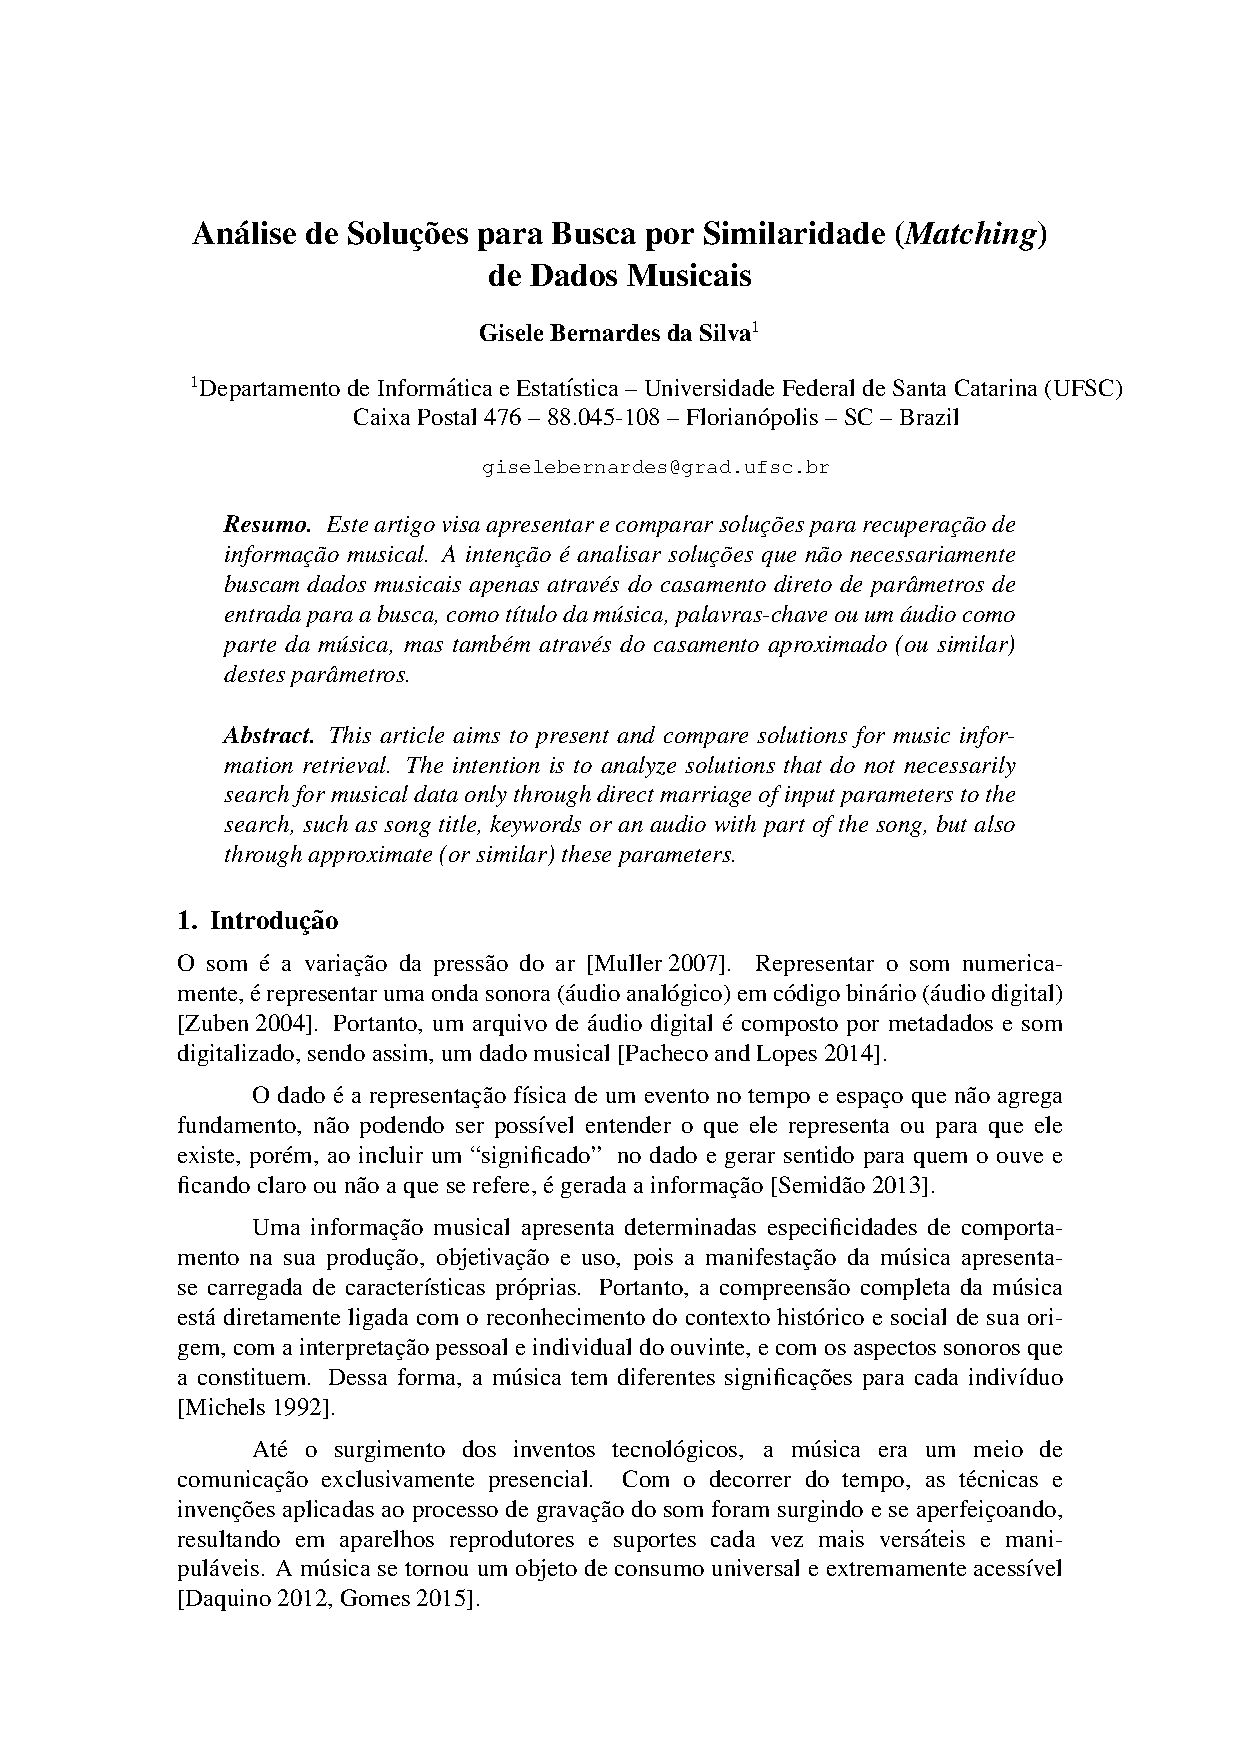
\includepdf[pages=-]{Artigo_Projetos2_GiseleBernardes.pdf}
%\anexo
\chapter{Anexo A} \label{anexoA}

%%%%%%%%%%%%%%%%%%%%%%%%%%%%%%%%%%%%%%%%%%%%%%%%%%%%%%%%%%%%%%%%%%%%%%%
% Fim do documento                                
\end{document}